\begin{figure*}[t]
\centering
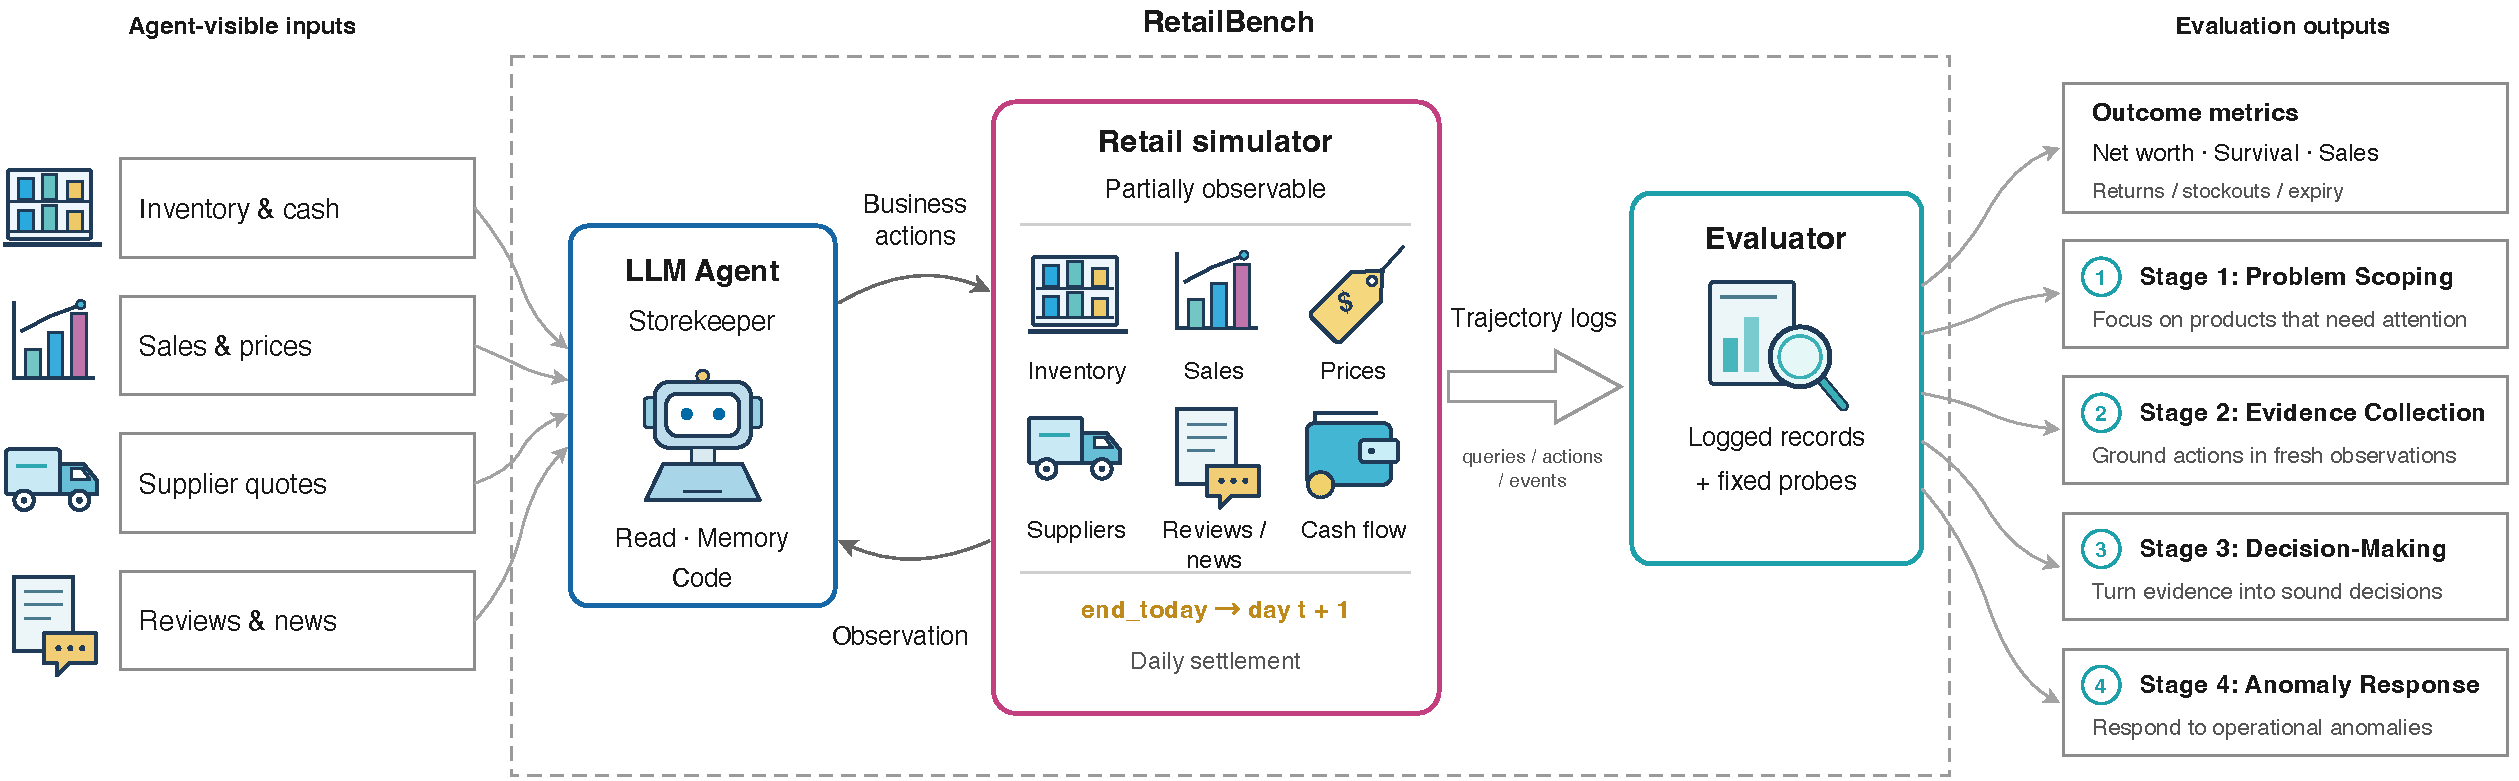
\includegraphics[width=0.96\textwidth]{figures/retailbench_framework.pdf}
\caption{RetailBench interaction framework. A tool-using LLM agent operates a partially observable, data-grounded retail simulator through information queries, auxiliary tools, and business actions. Agent trajectories are evaluated using operational outcomes and four-stage decision diagnostics.}
\label{fig:retailbench_framework}
\vspace{-3mm}
\end{figure*}

\paragraph{Retail, e-commerce, and supply-chain decision benchmarks.}
Prior work has investigated retail and supply-chain decision-making from several complementary perspectives. Retail simulation and promotion optimization study market dynamics and the effects of pricing and promotional strategies~\citep{xia2023retailsynth,xia2024simulationretailpromotions}. Demand recovery and transaction modeling characterize consumer behavior and purchasing patterns using empirical retail data~\citep{wang2025freshretailnet,tkachuk2024consumertransactions}. Web-shopping benchmarks evaluate agents on product search, navigation, and purchasing tasks~\citep{wang2025shoppingbench,3webshopscalablerealworldweb}, while supply-chain and inventory-control studies examine replenishment, resource allocation, and operational decision-making under dynamic constraints~\citep{OFCOURSE,inventory,leluc2023marlimmultiagentreinforcementlearning,invagentlargelanguagemodel,aimbenchevaluatingdecisionmakingbiases}. While these studies address important aspects of retail operations, many focus on individual decision problems rather than integrated, long-horizon business management (Table~\ref{tab:benchmark_axes}). RetailBench complements these efforts with a data-grounded, partially observable supermarket simulator that couples pricing, replenishment, supplier selection, and inventory management over extended horizons.

\paragraph{Long-horizon agent benchmarks.}
Recent benchmarks have extended LLM agent evaluation beyond short-horizon tasks to investigate sustained autonomy, long-term planning, and adaptation in complex environments. These efforts span ultra-long-horizon interactions and office workflows~\citep{utltabench,odysseybenchevaluatingllmagents}, virtual-world planning~\citep{herobenchbenchmarklonghorizonplanning}, lifelong experience reuse~\citep{zheng2025lifelongagentbench}, workplace task execution~\citep{xu2024theagentcompany}, and sustained business operations~\citep{backlund2025vendingbenchbenchmarklongtermcoherence,andonlabs2025vendingbench2}. Collectively, they examine complementary aspects of long-term agent behavior, including sequential planning, experience accumulation, and reliable execution over extended interactions. RetailBench complements these efforts by introducing a data-grounded, closed-loop benchmark for evaluating long-horizon agent performance in realistic business operations.
